\chapter{Application}
\label{chapter:application}


\section{Use cases}
\label{section:useCases}

Before diving into the application architecture and implementation details, let us first describe the use cases to get a complete overview of the functionality the app has to provide (See Fig. \ref{useCase}). The first and the most important use case is registering documents into the system. This would include automatically generating a registration number for each document. It is an important part of automating the current process, in which for registering a new document, the employee has to contact the registry administrator and ask for an available registration number. For the registration to be complete, the user has to specify a destination for the document. In most cases, the document would be internal, meaning that the destination would be other employees of the institution. In this case, the document is sent to the specified recipients, which receive an email notification and could then view the received documents in their account. However, some documents could have an external destination, like another institution or organization. In this case, the destination is specified so the document could be easily tracked in the future. Analogically, the issuer could specify an external source of the document, if it has one.

The user could upload an electronic version of the document, either immediately after the registration, or in any point of time in the future. Additionally, the upload feature is available for all recipients of a document.

The logic behind the document management process relies mainly on two actions: resolving and archiving a document. Basically, when a user receives a document, it means that he or she is expected to perform an action related to it. It could be an action as trivial as aknowledging that the document was received, or something more complex like reading and approving the document, uploading an edited version of the document or sending it further to other users. Regardless of this, the \textbf{resolve} action is meant to finalize the interaction between a user and a document.

\begin{figure}[H]
    \centering
    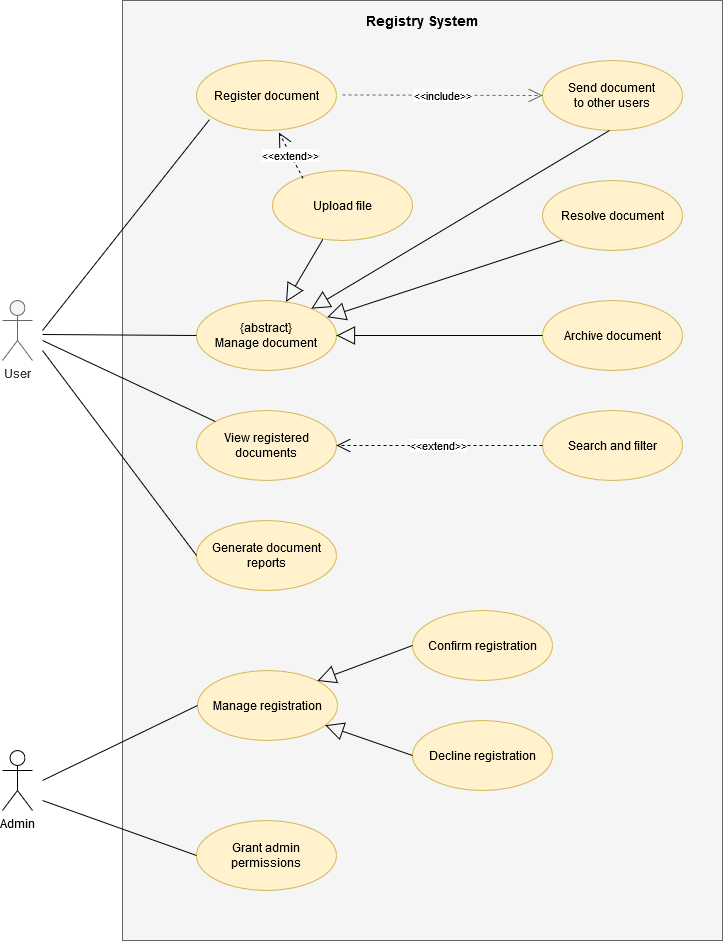
\includegraphics[width=5in]{images/useCase}
    \caption{Registry System Use Cases}
    \label{useCase}
\end{figure}

In simpler terms, marking a document as resolved is telling its issuer that all necessary actions from the receiver were taken.

The \textbf{archive} action, on the other hand, is meant to complete the document lifecycle and can only be performed by the document issuer. After a document is marked as archived, it could no longer get resolved or sent to other users. Resolving and archiving a document are closely related actions. After all, it seems rather logical that the user should only archive a document after it has been resolved by its receiver. However, the logic gets more complicated in case multiple receivers are specified. It could be that all of them have to take different actions on the document. It could also be that getting the document resolved by only one of them would be sufficient, if, for example, they are employees of the same department. In this case, getting a document resolved by a receiver is not a required constraint for the document to get archived. Similarily, when a document is resolved, it does not necessarily imply that it should immediately get archived. That is why we have not constrained the ability to archive a document based on its resolved status, but rather let the issuer do it when he or she deems it necessary. The \textit{Resolve document} and \textit{Archive document} use cases are described in detail in Table \ref{resolveUseCase} and \ref{archiveUseCase}.

\begin{table}[]
    \begin{tabular}{|p{0.3\textwidth}|p{0.6\textwidth}|}
        \hline
        Name                                  & Resolve document                                                  \\ \hline
        Short description                     & A user marks a document as resolved .                             \\ \hline
        Precondition                          & \begin{tabular}[c]{@{}l@{}}The user is logged in to the system.\\ The user is a receiver of the document.\end{tabular}                                         \\ \hline
        Postcondition                         & \begin{tabular}[c]{@{}l@{}}The document shows as resolved by the user in the app.\\ The document issuer receives an email notification.\end{tabular}                                         \\ \hline
        Error situations                      & The server could not perform the operation.                       \\ \hline
        System state in the event of an error & Document is not marked as resolved by the user.                   \\ \hline
        Actors                                & User                                                              \\ \hline
        Trigger                               & All document related actions needed from the user were performed. \\ \hline
        Standard process                      & \begin{tabular}[c]{@{}l@{}}(1) User selects the document.\\ (2) User introduces a resolve message (optional).\\ (3) User confirms the resolve action.\end{tabular}                                         \\ \hline
        Alternative process                   & (3') User cancels the resolve action.                             \\ \hline
    \end{tabular}
    \caption{Use case description for \textit{Resolve document}}
    \label{resolveUseCase}
\end{table}

\begin{table}[H]
    \begin{tabular}{|p{0.3\textwidth}|p{0.6\textwidth}|}
        \hline
        Name                                  & Archive document                                                                     \\ \hline
        Short description                     & A user marks a document as archived.                                                 \\ \hline
        Precondition                          & \begin{tabular}[c]{@{}l@{}}The user is logged in to the system.\\ The user is the issuer of the document.\end{tabular}                                                            \\ \hline
        Postcondition                         & \begin{tabular}[c]{@{}l@{}}The document shows as archived in the app.\\ The document cannot be send to other users or resolved.\end{tabular}                                                            \\ \hline
        Error situations                      & The server could not perform the operation.                                          \\ \hline
        System state in the event of an error & Document is not marked as archived by the user.                                      \\ \hline
        Actors                                & User                                                                                 \\ \hline
        Trigger                               & The document issuer considers that all actions related to the document are complete. \\ \hline
        Standard process                      & \begin{tabular}[c]{@{}l@{}}(1) User selects the document.\\ (2) User introduces an archiving message (optional).\\ (3) User confirms the archive action.\end{tabular}                                                            \\ \hline
        Alternative process                   & (3') User cancels the archive action.                                                \\ \hline
    \end{tabular}
    \caption{Use case description for \textit{Archive document}}
    \label{archiveUseCase}
\end{table}

Aside from managing owned and received documents, users should also have access to the entire register containing all documents cataloged into the sistem. This should include the ability to search for a specific document or filter the list based on different criteria. Another important feature would be generating a report in PDF or XLS that would either include all documents or only a certain subset matching the criteria specified by the user. The reports could then be printed and physically archived in the institution and should therefore replace the register that is currently filled out by hand.

Having a separate account for each user would imply the necessity of a registration process. As it is an internal app, a flow in which the user provides credentials and the account gets automatically created would not be sufficient. We have to also verify that the person requesting the account is an employee of the institution to which the application belongs. To achieve this, we would add the \textbf{Admin} role to our system. Admins would inherit all document management rights that the simple users have, but will also have special permissions that would allow them to manage the registration of new users.

\begin{figure}[H]
    \centering
    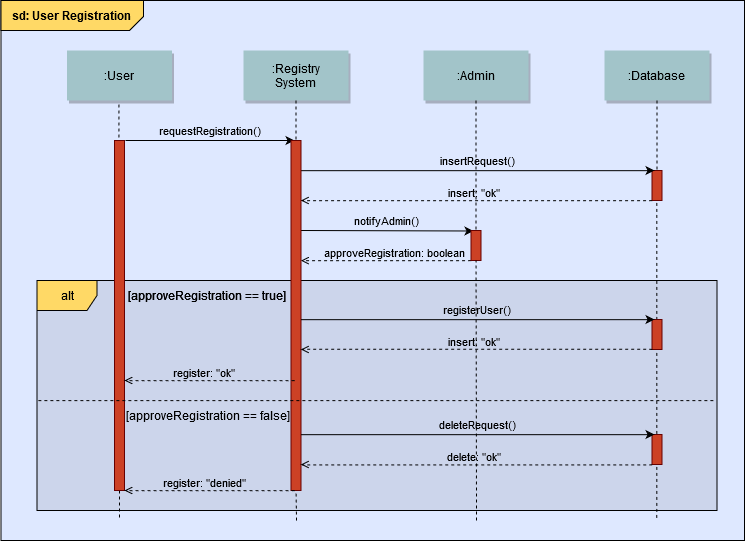
\includegraphics[width=5in]{images/sequenceDiagram}
    \caption{Sequence diagram for the \textit{User Registration} flow}
    \label{sequenceDiagram}
\end{figure}

As seen in Fig. \ref{sequenceDiagram}, the registration process begins with a user sending a request to the system to register a new account. The system then inserts the request into the database and sends an email notification to each of the Admins telling them that a new registration has been requested. The admins could then either confirm or decline the registration. In case of confirmation, the registration is completed within the database and the user is notified that the registration was successful. He or she can from that moment access the newly created account using the login credentials provided at the time of registration. In case an admin denies the registration, all information about the user is deleted from the database and a notification is sent to inform the user that his request was denied.



\section{Architecture}
\label{section:architecture}

The Registry System Application has a layered architecture (See Fig. \ref{deployment}) which closely follows the principles of layered architecture design described in \ref{subsection:layerArchitecture}.

\begin{figure}[H]
    \centering
    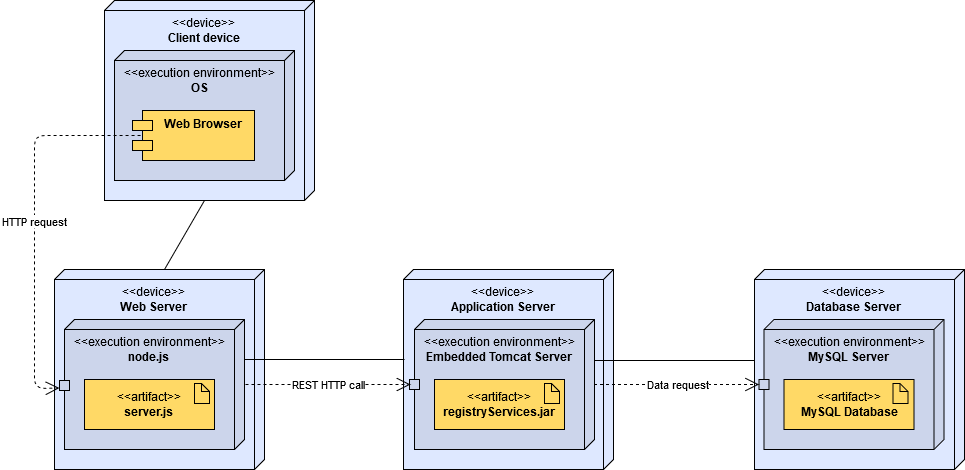
\includegraphics[width=6.5in]{images/deployment}
    \caption{Registry System Deployment Diagram}
    \label{deployment}
\end{figure}

\begin{itemize}
    \item The \textbf{persistence layer} is presented by a MySQL database. It connects to the application layer which queries the database for inserting, retrieving and updating data.
    \item The \textbf{application layer} is a Spring Boot Application, which defines the domain, encapsulates the business logic and exposes a REST API which is used by the presentation layer to manipulate the data.
    \item The \textbf{presentation layer} is a React JS application which connects to the Spring Boot backend through HTTP requests. The Web GUI can be accessed by the user on any device from a Browser.
\end{itemize}

In the following subsections, we are going to analize the architecture of each component in detail.



\subsection{Database}
\label{subsection:dbLayer}

Searching for a database schema that would support all required use cases, we came up with the design presented in Fig. \ref{db}. First of all, we have the \textbf{user} table, which, as the name suggests, will store information about the users of our app, like their name and department whitin the institution. An additional boolean field will be used to determine whether the user registration has been confirmed. The user table will also store authentication related data - the credentials the user provided at the moment of registration. One thing to mention here is that the password is encoded prior to storing it in the database using the \code{BCryptPasswordEncoder} provided by the Spring Security Framework. This assures that user passwords are not exposed even to persons that have direct access to the database.

\begin{figure}[H]
    \centering
    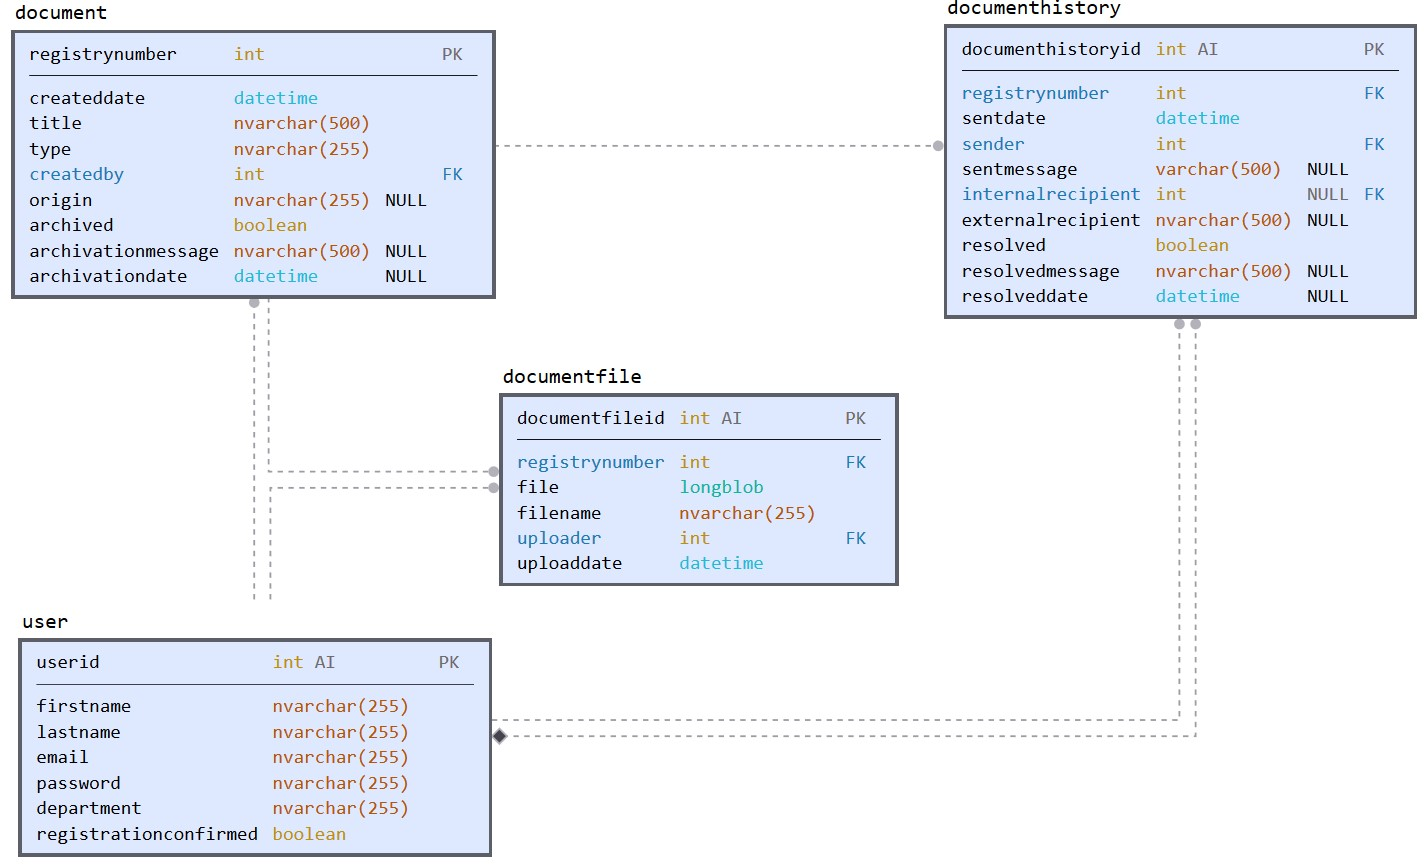
\includegraphics[width=6in]{images/db}
    \caption{Registry System Database Diagram}
    \label{db}
\end{figure}

The \textbf{document} table will store all registered documents, having the registry number as primary key. It is also the only primary key of this database that has no auto increment option set on it. Instead, we generate the next available number from code, each time a new document is registered into the system. This allows us more control over the way the number is generated. We already mentioned when describing use cases that a document can either be internal, or have external origin or destination, meaning that it is coming or should be sent to another institution. This information would be stored in the type field. One important thing to mention here is that a document cannot have external source and destination at the same time as it would technically not be related to the institution's registry anymore. That is why there are only three valid document types - internal, origin external and destination external. The table will also store a flag that will show the document's state as archived/not archived.

As an internal document could have multiple other users as recipients, another table is needed to store this m:n relationship. We decided to call this table \textbf{documenthistory}, as it reflects not only the recipients of a document, but also the \textit{resolved} status of the document set by a specific user. In case a document has external destination, only one entry for this document will be created in the documenthistory table, with the destination value stored in the \textit{externalrecipient} column.

Last but not least, we have a separate table for storing the uploaded files that represent the electronic version of the document. We only support uploading a single file per document now, but this has been kept as a separate table so that the design could support uploading multiple files if the feature would be desired in the future.



\subsection{Spring Boot Application}
\label{subsection:springBootApplication}

As we already mentioned, the backend logic of our Registry System is represented by a Spring Boot Application. It is divided in 4 independent modules which interact to provide the full functionality of the app.

\begin{itemize}
    \item The \textbf{Model} is the first module in this list. It defines the application domain, that is the classes that represent our use case, like \code{User} and \code{Document}.
    \item The \textbf{Persistence} module is the one that is responsible for interacting with the database. It defines and implements \textit{Repository} interfaces which retrieve, insert and update data using the Spring \code{NamedParameterJdbcTemplate} class. It also defines methods for mapping domain objects into JDBC parameters, as well as JDBC result sets into domain objects.
    \item The \textbf{Business} module is the biggest and most important one, because it encapsulates the business logic of the entire application. It defines and implements \textit{Service} interfaces which provide the necessary logic for the desired functionality. It is the module that is handling the server-side validation of user input, translation of the domain objects into Data Transfer Objects (DTOs), as well as mapping exceptions that occur throughout the program to user defined business exceptions. This is also the module that handles all the security related logic.
    \item The \textbf{Web} module contains \code{Controller} classes that define the REST API which will be used by the client. It maps a method to a specific URL (endpoint) that would be accessed in an HTTP request to trigger the method and defines the HTTP Response Status that should be returned.
\end{itemize}

For exception handling, we define a \code{@RestControllerAdvice} annotated class that will globally handle all exceptions that are thrown to the Controller layer (See \ref{controllerAdvice}). The way this works is that in this class we define a method for each exception type that could occur. This method then gets called each time an exception of that type is thrown. Just imagine that five different methods can throw an \code{EntityNotFoundException}. Instead of handling all those five cases separately, we only define a single method which returns a meaningful error message and the 404 HTTP status. In this way we centralize the place where errors are handled which provides better readability and significantly reduces the amount of repetitive boilerplate code.

\begin{lstlisting}[language=Java, caption={Simplified example of global exception handling class}, label={controllerAdvice}]

@RestControllerAdvice
public class ControllerExceptionHandler {

    @ExceptionHandler(EntityNotFoundException.class)
    @ResponseStatus(HttpStatus.NOT_FOUND)
    public ErrorResponse handleException(EntityNotFoundException e) {
        return new ErrorResponse(e.getMessage(), e.getCause());
    }

    //other @ExceptionHandler methods follow
}

\end{lstlisting}

With the same goal of reducing boilerplate code in mind, we have used the \textbf{Lombok} java library which provides great shortcuts in form of annotations for most used java code snippets. As an example, we used the \code{@Data} annotation on our model classes, which generates all the repetitive code that is normally associated with simple POJOs (Plain Old Java Objects) and beans: getters for all fields, setters for all non-final fields, toString, equals and hashCode implementations involving the fields of the class, and a constructor that initializes all required arguments. Another feature that we used from Lombok is the \code{@Slf4j} annotation, which automatically generates a Logger associated to the class it is used on.

An important part of the application is the security logic implemented using the features provided by the Spring Security framework. An unauthenticated user would have access only to the registration and login pages. All other endpoints would need a valid JWT token to be accessed. In some cases it matters not only \textit{if} the user is authenticated, but also \textit{who} the user is. A good example is the \code{archiveDocument} endpoint which should only be called by the document issuer. All the other users are unauthorized to perform this method on that specific document. In that case, in addition to the JWT token validation, we need to manually verify the user's identity. Of course, after integrating the backend with the frontend app, a user won't have any way of triggering an unauthorized endpoint from the UI. For instance, we won't display \textit{Archive} buttons for documents issued by another users as the one that is currently logged in. However, the Spring Boot app is a standalone application that should not necessarily be tied to the frontend. Its endpoints could be triggered by directly accessing the URL they are associated with. This is why it is important to perform server-side validations such as verifying the identity of a user that is performing a request.



\subsection{ReactJS Application}
\label{subsection:reactJsApplication}

The presentation layer of our Registry System is represented by a ReactJS application with Redux as a state container. The whole application state is kept into a global \textit{store}, making the app behavior predictable and easy to understand. REST HTTP requests sent to the backend are performed by the Redux \textit{actions}, keeping data fetching code separate from the other logic. The retrieved data is then passed to the \textit{reducers}, which update the application state. It is worth mentioning that with this approach, each time a reducer updates something from the application state that is showing on the currently displayed page, the page automatically rerenders, meaning that it updates the displayed information. This assures that the data displayed is always up-to-date without the necessity of a refresh or other interaction from the client.

For building the UI, we used the \textbf{React Bootstrap} frontend library. It integrates the classical Bootstrap stylesheets into ready to use react components that follow the latest UI trends. Bootstrap was designed for developing responsive and mobile-first websites. We took advantage of this feature to custumize our UI so that it would be accessible from all kinds of devices, from mobile to tablets to PCs. In the following subsection, while providing screenshots for some of the app pages, we will sometimes include both the PC and mobile version to demonstrate how the app adapts to different screen sizes.


\section{Implementation}
\label{section:implementation}


